
\begin{figure}
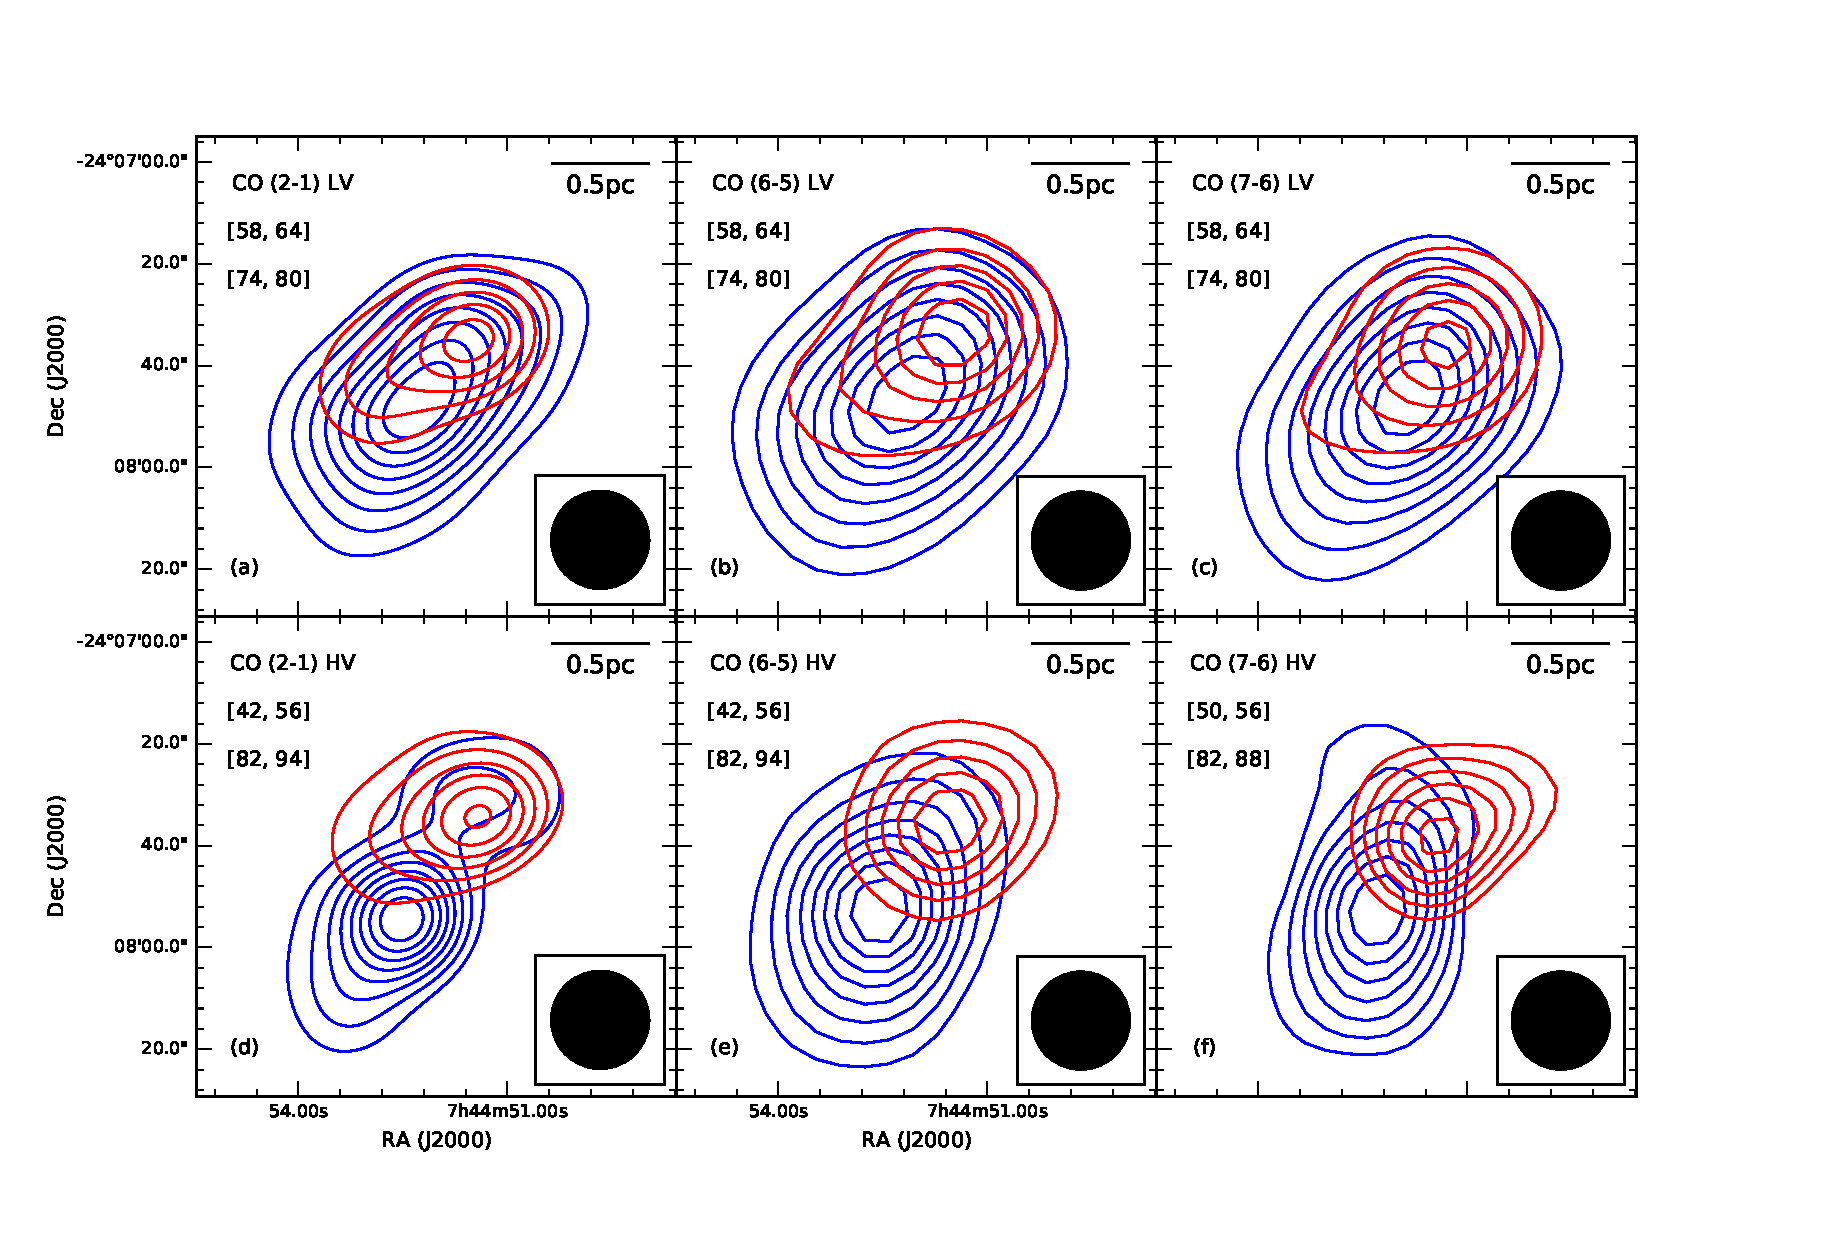
\includegraphics[scale=.6]{./fig/cvl_contour.eps}
\caption{(a)-(c) Low-velocity emission of reconstructed CO J = (2-1), (6-5), (7-6) lines, with velocity range 58 to 64 km s$^{-1} $ and 74 to 80 km s$^{-1}$ for the blueshifted lobe (blue) and the redshifted lobe (red); (d)-(e) High-velocity emission of reconstructed CO J = (2-1), (6-5) lines, with velocity range 42 to 56 km s$^{-1} $ and 82 to 94 km s$^{-1}$ for the blueshifted lobe (blue) and  the redshifted lobe (red); (f) High-velocity reconstructed CO J = (7-6) emission, with velocity range 50 to 56 km s$^{-1} $ and 82 to 88 km s$^{-1}$ for the blueshifted lobe (blue) and  the redshifted lobe (red). For (a)-(e), the contour levels are starting from 20\% and at steps of 10\%. For (f), the contour levels are starting from 30\% and at steps of 10\%. The central stars mark the position of the millimeter sources detected by \citet{2009ApJ...696...66Q}.  \label{fig2}}
\end{figure}



However, we found the best fitting result at most velocities has a $\chi^2_{red}$ less than 1, indicating we might be a bit conservative at . So we adjusted the intensity uncertainties with a appropriate factor to 



Since the $^{13}$CO emission is not detected in the outflowing gas, the four transitions of $^{12}$CO are assumed to be 
optically thin during our analysis. 